\exer{Évaluation d’une expression parenthésée}


Dans un éditeur l'ajout d'une parenthèse fermante surnuméraire est signalé (mise en surbrillance). La construction d'un vérificateur de parenthèses repose sur l'utilisation de piles.

\begin{figure}[hbt]
	\begin{center}
		\begin{minipage}[t]{0.32\textwidth}
			\centering
			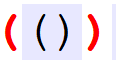
\includegraphics[height=0.2\textwidth]{notepadppB}
			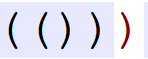
\includegraphics[height=0.2\textwidth]{notepadppPB}
			\caption{Éditeur généraliste Notepad++}
		\end{minipage}
		\hfill
		\begin{minipage}[t]{0.32\textwidth}
			\centering
			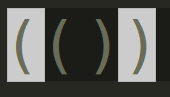
\includegraphics[height=0.2\textwidth]{pyzoB}
			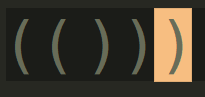
\includegraphics[height=0.2\textwidth]{pyzoPB}
			\caption{Éditeur Python Pyzo}
		\end{minipage}
		\hfill
		\begin{minipage}[t]{0.32\textwidth}
			\centering
			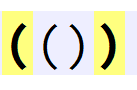
\includegraphics[height=0.2\textwidth]{texStudioB}
			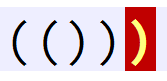
\includegraphics[height=0.2\textwidth]{texStudioPB}
			\caption{Éditeur LaTeX TeXstudio}
		\end{minipage}
		\caption{Expressions bien et mal parenthésées dans différents éditeurs}
	\end{center}
\end{figure}

Nous allons considérer 3 types de ponctuations symétriques~: 
\begin{itemize}
	\item les parenthèses \texttt{(} et \texttt{)}~; 
	\item les crochets \texttt{[} et \texttt{]}~; 
	\item les accolades \texttt{\{} et \texttt{\}}~; 
\end{itemize}

On souhaite savoir reconnaitre 4 cas différents~: 
\begin{itemize}
	\item fermeture sans ouverture préalable~; 
	\item fermeture par le mauvais type de parenthèse~; 
	\item une ouverture sans fermeture~; 
	\item l'expression est bien parenthésée. 
\end{itemize}


%On donne un fichier texte par numéro d'anonymat \texttt{alpha} à télécharger sur le site de la classe et à mettre dans le même répertoire que votre script. Ce fichier est appelé 'expression$\_$parenthesee$\_$i.txt' avec \texttt{i=alpha}. C'est une expression sensé être mathématique et bien parenthésée.
%
%On donne la fonction \texttt{def charger$\_$expression$\_$parenthesee(alpha:int) -> str:} qui pour votre numéro alpha charge l'expression correspondante.
%
%\begin{lstlisting}
%def charger_expression_parenthesee(alpha):
%    with open('expression_parenthesee_'+str(alpha)+'.txt','r') as f:
%        code=f.read()
%    return code
%\end{lstlisting}
%
%\question{} Charger votre expression parenthésée et donner sa taille.
%
%\question{} Donner le nombre de parenthèses '(' dans cette expression. 

Nous allons commencer par nous occuper dans un premier temps uniquement d'un seul type de ponctuations~: les parenthèses. 

\question{Écrire une fonction \texttt{verifPar0(texte)} qui prend en entrée une chaine de caractères et renvoie~: }
\textit{\begin{itemize}
	\item le nombre d'ouvertures non-fermées~;
	\item \texttt{-1} dès qu'on rencontre une fermeture sans ouverture préalable.
\end{itemize}}

Une pile sera initialisée au début de la fonction~: on ajoutera l'ouverture dans la pile qu'on dépilera lorsqu'il y a fermeture de la parenthèse avec le même type.

\question{Tester la fonction avec \texttt{"(()())"}, \texttt{"(()()"} et \texttt{"(()()))"}.}

Nous ajoutons ici les autres types de ponctuations~: il faut donc vérifier si la fermeture correspond bien à l'ouverture dans ce cas-là. 

\question{Écrire une fonction \texttt{verifPar1(texte)} qui prend en entrée une file remplie de caractère et renvoie~: }
\textit{
\begin{itemize}
	\item le nombre d'ouvertures non-fermées~; 
	\item \texttt{-1} dès qu'on rencontre une fermeture sans ouverture préalable~; 
	\item \texttt{c} dès qu'on rencontre une erreur de type au caractère \texttt{c}.
\end{itemize}}

\question{Tester la fonction avec \texttt{"\{[()\}"}, \texttt{"\{[()]"} et \texttt{"\{[()]\}"}.}

%
%\question{} Tester avec le texte contenu dans  expression$\_$parenthesee$\_$i.txt.
